\documentclass[tikz]{standalone}

\begin{document}
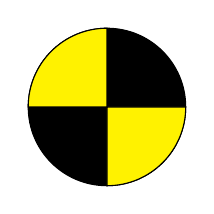
\begin{tikzpicture}
  \draw[fill=black] (0, 0) circle (1);
  \draw[fill=yellow] (0, 0) -- (1, 0) arc (0:-90:1) -- cycle;
  \draw[fill=yellow] (0, 0) -- (-1, 0) arc (180:90:1) -- cycle;
\end{tikzpicture}


\begin{tikzpicture}
  \draw[fill=black] (0, 0) circle (1);
  \draw (0,0) node[yellow,anchor=center]{\Huge\textbf{\textsf{PDF}}};

  \clip (0, 0) -- (1, 0) arc (0:-90:1) -- (0, 0) -- (-1, 0) arc (180:90:1) -- cycle;
  \draw[fill=yellow] (0, 0) circle (1);
  \draw (0,0) node[black,anchor=center]{\Huge\textbf{\textsf{PDF}}};
\end{tikzpicture}
\end{document}
